
\documentclass[11pt]{article}
\usepackage[a4paper,margin=2.2cm]{geometry}
\usepackage{graphicx}
\usepackage{booktabs}
\usepackage{array}
\usepackage{longtable}
\usepackage{adjustbox}
\usepackage{float}
\usepackage{caption}
\usepackage{hyperref}
\usepackage{amsmath, amssymb}
\usepackage{enumitem}
\usepackage{xcolor}
\setlength{\parindent}{0pt}
\setlength{\parskip}{0.65em}
\captionsetup{font=small,labelfont=bf}
\hypersetup{colorlinks=true,linkcolor=black,urlcolor=blue,citecolor=black}

\newcommand{\conclusionbox}[1]{\vspace{0.3em}\noindent\fbox{\begin{minipage}{0.96\linewidth}#1\end{minipage}}\vspace{0.4em}}

\title{Ovule-number project: data structure, model-readiness, and analysis plan}
\author{Prepared for Daniel Ortiz-Barrientos}
\date{8 June 2026}

\begin{document}
\maketitle

\section*{Purpose}

This report characterises the files supplied for the ovule-number project and asks a practical question: which parts of the data can test a model linking ovule number, reproductive isolation, genetic distance, life history, mating system, and phylogenetic structure? I treat Table 1 as the pairwise reproductive-isolation and cross-outcome table, Table 2 as the curated lineage-level covariate table, Table 2b as the master ovule-number database, the genetic-distance table as pair-level divergence information, and the Newick file as the phylogenetic structure for the phylogenetically independent pairs.

The working model assumed here is not a single fitted equation. It is the data structure needed to test whether ovule number, or contrasts in ovule number between species, predict cross success or reproductive isolation once genetic distance, mating system, life history, measurement type, and phylogenetic non-independence are controlled. This matters because the same biological idea can be tested in two different ways. A pair-level test asks whether species pairs with larger ovule-number contrasts have larger RI. A directional test asks whether the outcome differs when the many-ovule species is the maternal parent rather than the paternal parent. The second test is closer to the mechanism, but it needs reciprocal cross data on the right scale.

\conclusionbox{\textbf{Main result.} The data are already close to a useful comparative analysis. After removing rows flagged for removal, there are 560 retained Table 1 rows and 133 retained rows with \texttt{PI\_name}. The most conservative complete-case subset with PI status, both ovule numbers, and nonmissing K2P distance contains 87 pairs. If both ovule estimates are restricted to confidence categories 1--2, this decreases to 57 pairs.}

\begin{figure}[H]
\centering
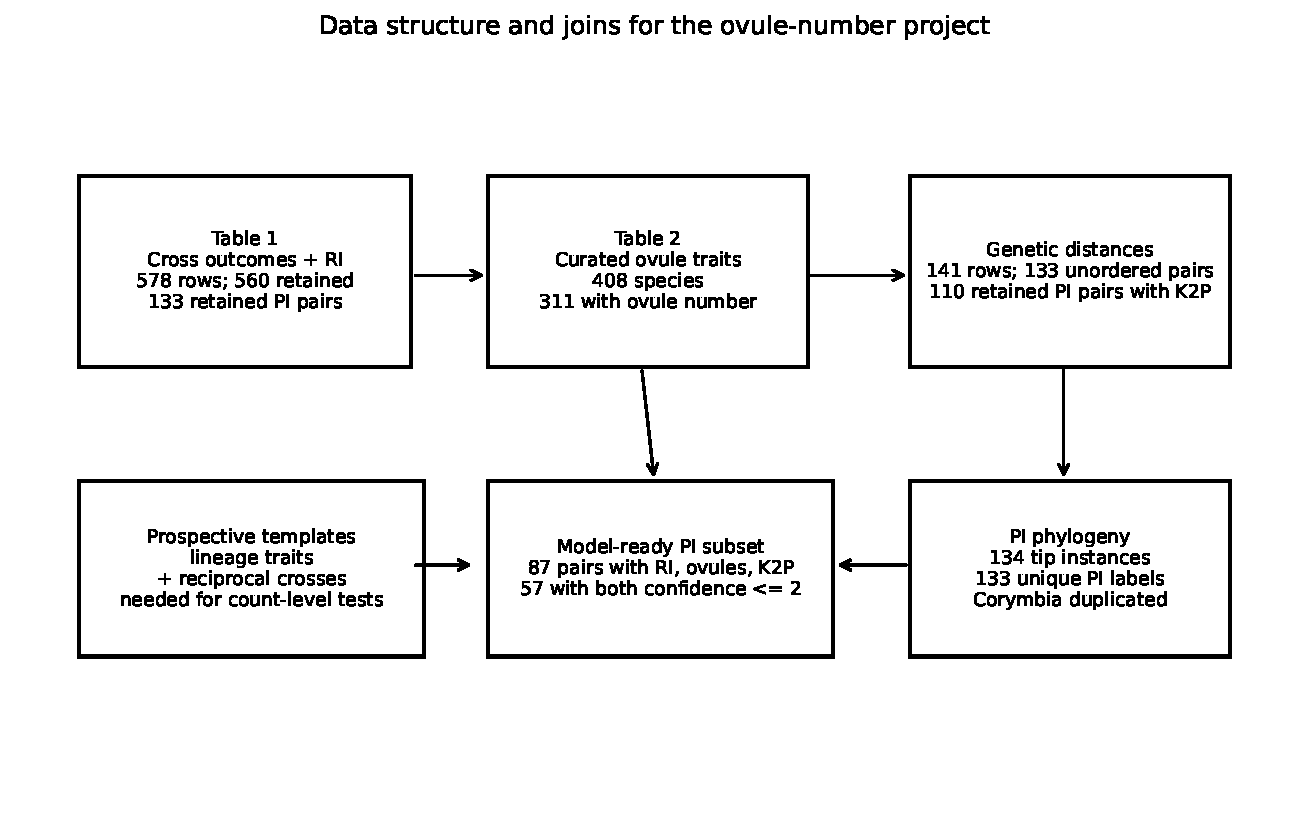
\includegraphics[width=0.98\linewidth]{../figures/fig1_data_map.pdf}
\caption{Overview of the supplied data files and the main joins needed for model testing.}
\end{figure}

\section*{Data inventory}

\begin{table}
\caption{Input files and their modelling roles.}
\label{tab:dataset_inventory}
\begin{adjustbox}{max width=\textwidth}
\begin{tabular}{lllllll}
\toprule
dataset & role & rows & columns & families & genera & unique\_species \\
\midrule
Table1\_2026\_01\_09.csv & Pairwise cross outcomes and RI & 578 & 15 & 50 & 93 & 410 \\
Table2\_2025\_12\_15.csv & Curated ovule, life-history, and mating-system covariates & 408 & 6 &  & 94 & 408 \\
Table2b\_2025\_11\_25.csv & Ovule-number master table before final curation & 5496 & 7 & 309 & 1840 & 3789 \\
Genetic\_distances\_results.csv & K2P genetic distances for PI species pairs & 141 & 3 &  &  & 266 \\
All\_PI\_pairs\_Zuntini\_2025\_10.tre & Phylogeny over PI-pair labels & 134 &  &  &  & 133 \\
\bottomrule
\end{tabular}
\end{adjustbox}
\end{table}


Table 1 contains the response variables: reciprocal intraspecific and interspecific cross outcomes, hybrid proportions for pollen-competition rows, RI, and measurement type. Table 2 contains the main lineage-level predictors: ovule number, confidence in the estimate, life history, and mating system. Table 2b is valuable as provenance and as a source for future curation, but Table 2 is the better analysis table because it supplies one best estimate per species.

A small naming issue should be fixed before formal analysis. The column-description file refers to a \texttt{PI} column, but the uploaded Table 1 does not contain a separate \texttt{PI} column. It contains \texttt{PI\_name}. I therefore treated a nonmissing \texttt{PI\_name} as the operational PI flag in this audit. That is reasonable for now because the retained PI rows and the tree labels agree, but I would add an explicit Boolean column called \texttt{is\_PI} before modelling.

\begin{table}
\caption{Important structural features of Table 1.}
\label{tab:table1_quality}
\begin{adjustbox}{max width=\textwidth}
\begin{tabular}{lll}
\toprule
quantity & count & comment \\
\midrule
All pair rows & 578 & Before applying remove flag \\
Retained pair rows & 560 & remove == no \\
Rows flagged for removal & 18 & Duplicates or lower-quality alternatives \\
Rows with PI\_name & 141 & Available proxy for PI flag \\
Retained PI rows & 133 & remove == no and PI\_name present \\
Unique PI names retained & 133 & Should map to phylogeny tips \\
Negative RI values & 59 & Interspecific performance can exceed intraspecific baseline \\
RI values equal to 1 & 143 & Boundary values affect beta regression \\
\bottomrule
\end{tabular}
\end{adjustbox}
\end{table}


\section*{Coverage and model readiness}

The most important structural result is the cascade from all retained cross rows to complete model-ready rows. Table 2 matches all retained Table 1 species by exact binomial names, but not all Table 2 rows have a numeric ovule estimate. The genetic-distance file covers the PI pairs, but 23 rows have missing K2P values. These two sources of missingness define the effective sample size for the strongest test.

\begin{figure}[H]
\centering
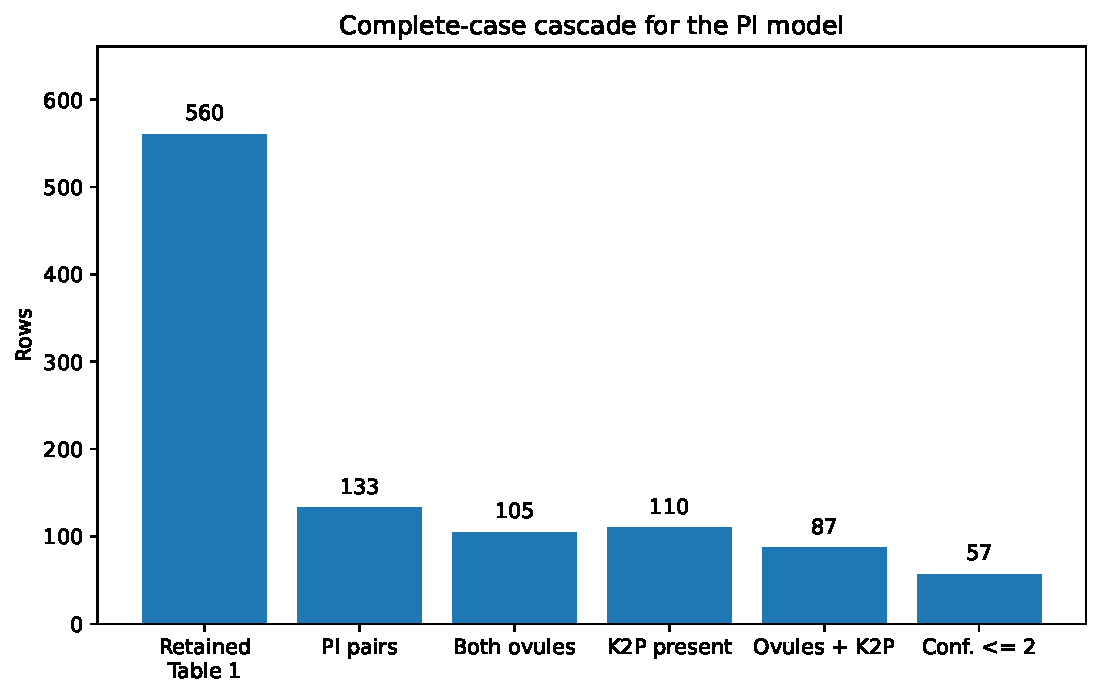
\includegraphics[width=0.82\linewidth]{../figures/fig2_model_readiness_cascade.pdf}
\caption{The effective sample size after imposing phylogenetic independence, ovule-number availability, K2P availability, and high-confidence ovule estimates.}
\end{figure}

\begin{table}
\caption{Join coverage across cross, ovule, and genetic-distance data.}
\label{tab:join_coverage}
\begin{adjustbox}{max width=\textwidth}
\begin{tabular}{lllllllll}
\toprule
subset & rows & both\_species\_in\_Table2 & both\_ovules\_numeric & K2P\_row\_present & K2P\_nonmissing & both\_ovules\_and\_K2P & both\_ovules\_K2P\_conf\_le\_3 & both\_ovules\_K2P\_conf\_le\_2 \\
\midrule
All Table1 rows & 578 & 577 & 448 & 141 & 118 & 94 & 93 & 61 \\
Retained Table1 rows & 560 & 560 & 434 & 133 & 110 & 87 & 86 & 57 \\
Retained PI rows & 133 & 133 & 105 & 133 & 110 & 87 & 86 & 57 \\
\bottomrule
\end{tabular}
\end{adjustbox}
\end{table}


The retained PI subset contains 133 rows. Of these, 105 have both ovule numbers and 110 have nonmissing K2P distances. The intersection is 87 rows. This means a complete-case PI analysis is feasible, but it will have limited power for interactions among ovule number, genetic distance, mating system, life history, and measurement type. The model should therefore start simple and add complexity only when the residual structure justifies it.

\begin{table}
\caption{Readiness by cross-outcome measure.}
\label{tab:measure_readiness}
\begin{adjustbox}{max width=\textwidth}
\begin{tabular}{llllllllll}
\toprule
measure & retained\_rows & PI\_rows & both\_ovules & nonmissing\_K2P & complete\_PI\_K2P\_ovules & RI\_mean & RI\_median & RI\_min & RI\_max \\
\midrule
fruit set & 146 & 26 & 119 & 24 & 20 & 0.62 & 0.794 & -0.379 & 1 \\
pollen competition & 18 & 12 & 14 & 11 & 9 & 0.443 & 0.438 & -0.897 & 1 \\
seed number per fruit & 77 & 13 & 54 & 12 & 9 & 0.52 & 0.478 & -0.164 & 1 \\
seed set & 319 & 82 & 247 & 63 & 49 & 0.529 & 0.531 & -0.628 & 1 \\
\bottomrule
\end{tabular}
\end{adjustbox}
\end{table}


Measurement type is a major source of heterogeneity. Fruit set, seed set, seed number per fruit, and pollen competition are not the same response. They differ in the biological process measured and in the denominator. Fruit set measures whether a fruit forms. Seed set includes failed crosses when expressed as seeds per pollination. Seed number per fruit excludes failed crosses. Pollen competition uses hybrid proportions rather than direct seed or fruit counts. Pooling these four responses without a measurement-type term would mix mechanisms and can create regression slopes that are hard to interpret.

\begin{figure}[H]
\centering
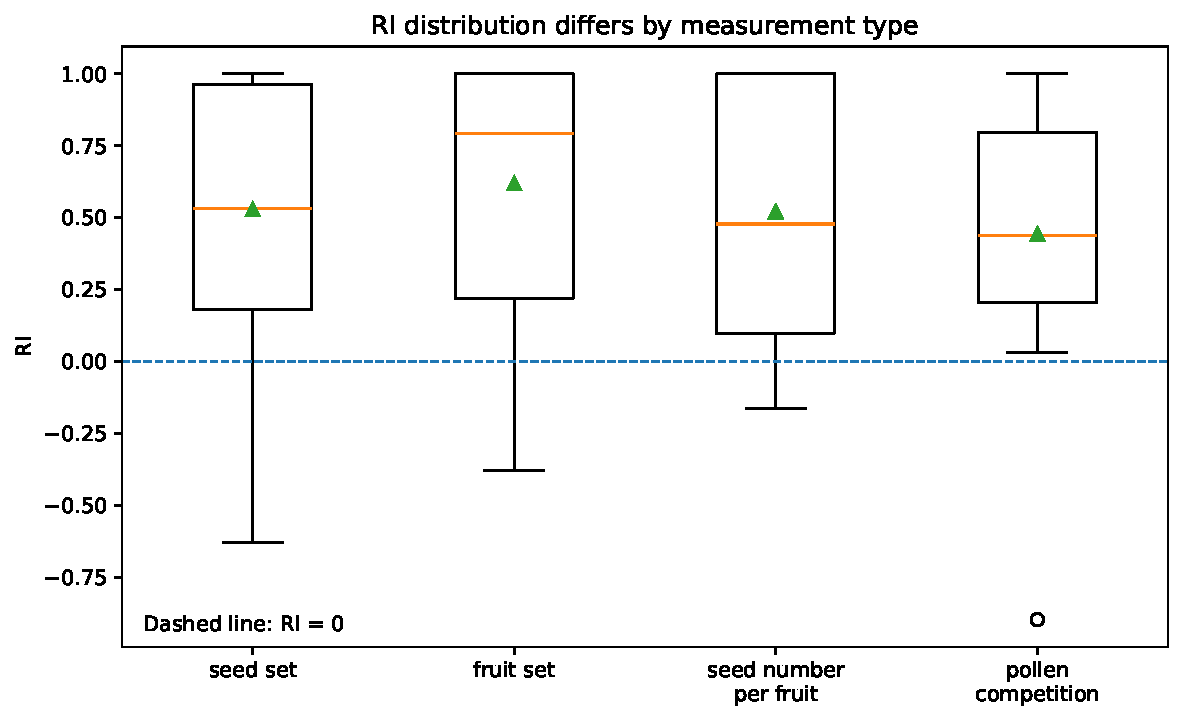
\includegraphics[width=0.86\linewidth]{../figures/fig4_RI_by_measure.pdf}
\caption{RI values by measurement type among retained Table 1 rows. The distributions differ enough that measurement type should be modelled, stratified, or treated as a sensitivity factor.}
\end{figure}

\section*{Ovule-number data}

Table 2 contains 408 species. Numeric ovule estimates are present for 311 species and missing for 97. Confidence is useful because it gives a simple way to separate species-level estimates from weaker genus-level or indirect estimates. Most missing ovule numbers are in confidence categories 4 and 5.

\begin{table}
\caption{Ovule-number coverage by confidence category.}
\label{tab:confidence_summary}
\begin{adjustbox}{max width=\textwidth}
\begin{tabular}{llllll}
\toprule
confidence & species & ovule\_numbers\_present & ovule\_numbers\_missing & median\_ovules & max\_ovules \\
\midrule
1 & 208 & 208 & 0 & 21.56 & 9478 \\
2 & 16 & 16 & 0 & 4 & 4 \\
3 & 85 & 85 & 0 & 106 & 2000 \\
4 & 67 & 2 & 65 & 3500000 & 3500000 \\
5 & 32 & 0 & 32 &  &  \\
\bottomrule
\end{tabular}
\end{adjustbox}
\end{table}


\begin{figure}[H]
\centering
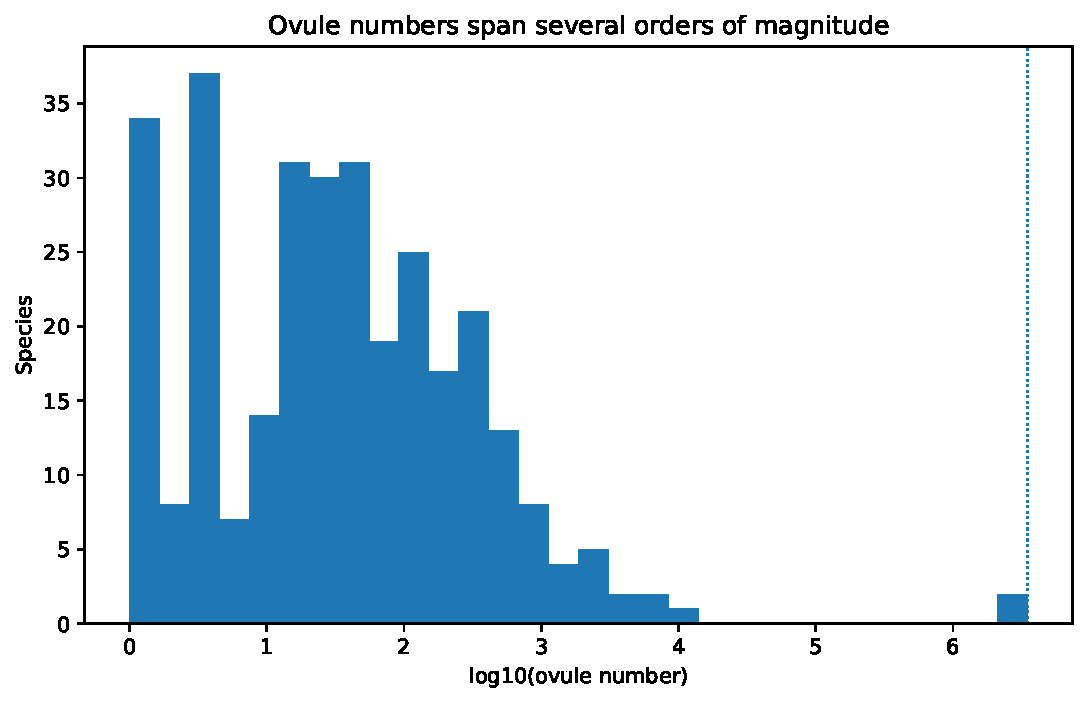
\includegraphics[width=0.82\linewidth]{../figures/fig5_ovule_number_distribution.pdf}
\caption{Ovule numbers are highly skewed, so model terms based on ovule number should use a log scale. The two largest estimates are low-confidence values and should be checked in sensitivity analyses.}
\end{figure}

\begin{figure}[H]
\centering
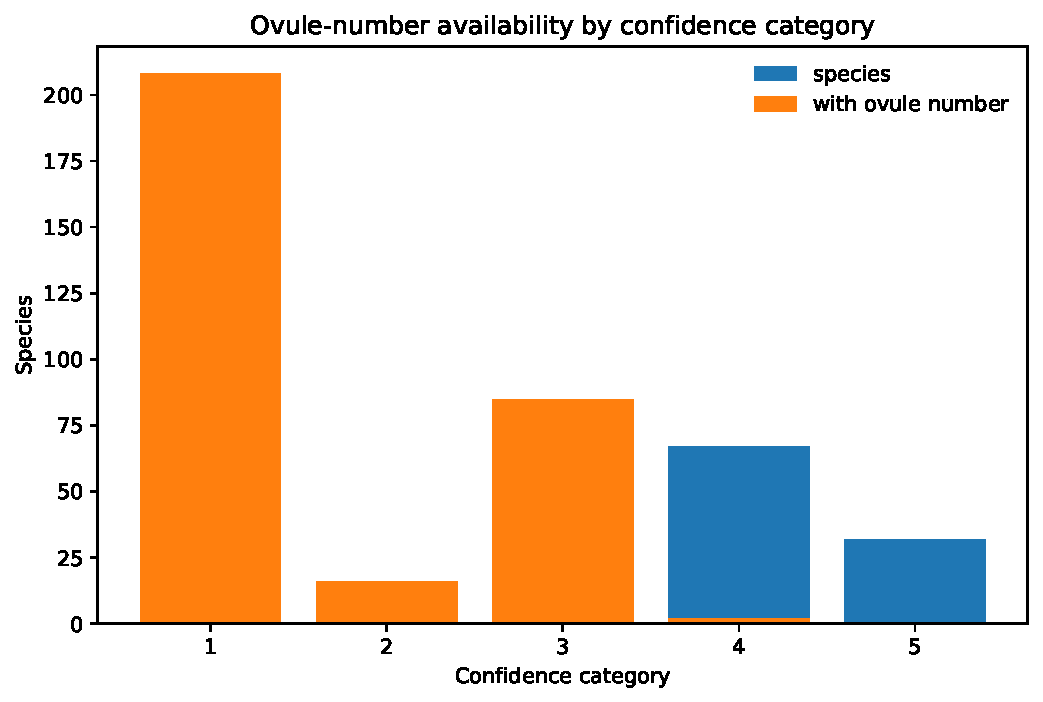
\includegraphics[width=0.78\linewidth]{../figures/fig6_confidence_coverage.pdf}
\caption{Ovule-number availability by confidence category. Confidence categories 1--3 carry nearly all numeric ovule estimates.}
\end{figure}

\begin{table}
\caption{Largest ovule-number estimates in Table 2.}
\label{tab:largest_ovules}
\begin{adjustbox}{max width=\textwidth}
\begin{tabular}{lllll}
\toprule
species & ovule\_number & confidence & life\_history & mating\_system \\
\midrule
Cattleya sincorana & 3500000 & 4 & perennial & outcrossing \\
Cattleya pfisteri & 3500000 & 4 & perennial & outcrossing \\
Orchis provincialis & 9478 & 1 & perennial & mixed-mating \\
Dactylorhiza incarnata & 7756 & 1 & perennial & mixed-mating \\
Platanthera chlorantha & 5831 & 1 & perennial & mixed-mating \\
Neotinea tridentata & 4452 & 1 & perennial & outcrossing \\
Platanthera bifolia & 4004 & 1 & perennial & mixed-mating \\
Dactylorhiza maculata & 2605.178 & 1 & perennial & mixed-mating \\
Nicotiana longiflora & 2367.92 & 1 & perennial & mixed-mating \\
Erythranthe lutea & 2140.32 & 1 & perennial & mixed-mating \\
Cyrtandra kauaiensis & 2000 & 3 & woody & outcrossing \\
Gymnadenia conopsea & 2000 & 3 & perennial & mixed-mating \\
Nicotiana alata & 1732 & 3 & perennial & outcrossing \\
Cyrtandra platyphylla & 1700 & 3 & woody & outcrossing \\
Nicotiana plumbaginifolia & 1538.48 & 1 & annual & selfing \\
\bottomrule
\end{tabular}
\end{adjustbox}
\end{table}


The main modelling consequence is simple. Raw ovule number should not enter the model linearly. It spans several orders of magnitude, and a few taxa can dominate raw-scale fits. Use \(\log_{10}(O)\), where \(O\) is ovule number, and then construct biologically interpretable contrasts such as
\[
\Delta O = \left| \log_{10}(O_1) - \log_{10}(O_2) \right|,
\]
for pair-level analyses, and
\[
D_{m,p} = \log_{10}(O_m) - \log_{10}(O_p),
\]
for directional analyses, where \(m\) and \(p\) denote maternal and paternal species.

\section*{Genetic distance and phylogeny}

\begin{table}
\caption{Summary of genetic-distance data.}
\label{tab:gd_summary}
\begin{adjustbox}{max width=\textwidth}
\begin{tabular}{lll}
\toprule
quantity & count & comment \\
\midrule
Rows in genetic-distance table & 141 &  \\
Unique unordered species pairs & 133 & Duplicates are identical for eight pairs \\
Rows with missing K2P & 23 &  \\
Rows with nonmissing K2P & 118 &  \\
Median nonmissing K2P & 0.012 &  \\
Maximum nonmissing K2P & 0.291 &  \\
\bottomrule
\end{tabular}
\end{adjustbox}
\end{table}


The genetic-distance table has 141 rows and 133 unique unordered species pairs. Eight species pairs are duplicated in the file; the duplicated distances are identical in this audit, so they do not change the values, but they should still be collapsed before modelling. The larger issue is missing distance values: 23 rows have no K2P value. Because the retained PI cross rows all have a corresponding distance-table row, the missingness is not a join problem. It is a missing-value problem.

\begin{table}
\caption{Summary of PI-name matching to the phylogeny.}
\label{tab:tree_summary}
\begin{adjustbox}{max width=\textwidth}
\begin{tabular}{ll}
\toprule
metric & value \\
\midrule
tip instances & 134 \\
unique tip labels & 133 \\
duplicated tip labels & 1 \\
PI names in clean Table1 & 133 \\
PI names found in tree & 133 \\
PI names missing from tree & 0 \\
\bottomrule
\end{tabular}
\end{adjustbox}
\end{table}


The tree is nearly aligned with the PI structure. All retained \texttt{PI\_name} labels are present in the tree. However, the tree contains 134 tip instances but only 133 unique tip labels; the duplicated tip label is \texttt{Corymbia}. Many phylogenetic comparative tools require unique tip labels. Before fitting phylogenetic models, this duplicate label should be resolved, either by renaming the tips with unique suffixes or by checking whether one occurrence is unintended.

\section*{What the current data can test}

The pair-level test is ready for a first analysis. The clean dataset \texttt{model\_ready\_PI\_pairs.csv} contains 87 rows with RI, both ovule numbers, and K2P distance. A useful first model would be
\[
RI_i = \alpha + \beta_1 \log_{10}(d_i + c) + \beta_2 \Delta O_i + \beta_3 \bar O_i + \gamma_{measure(i)} + \varepsilon_i,
\]
where \(d_i\) is genetic distance, \(c\) is a small constant if zero distances are retained, \(\Delta O_i\) is the absolute log ovule-number contrast, \(\bar O_i\) is the mean log ovule number of the pair, and \(\gamma_{measure(i)}\) is a measurement-type effect. I would not start with all life-history and mating-system interactions because the complete-case PI subset is too small for that many terms.

\begin{figure}[H]
\centering
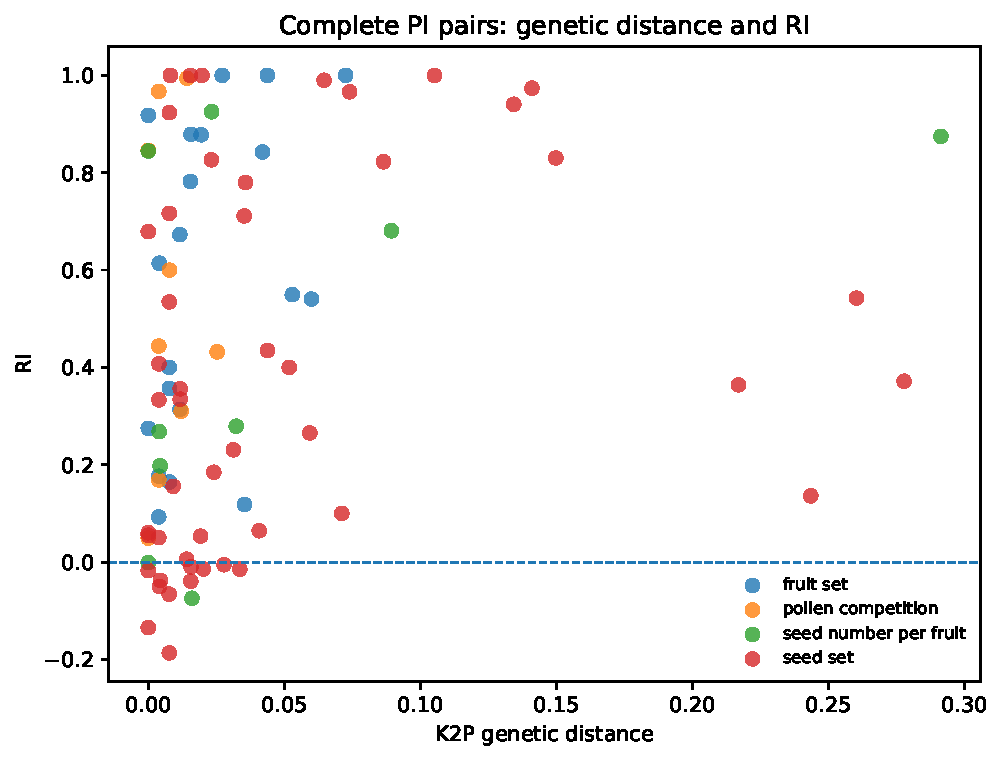
\includegraphics[width=0.80\linewidth]{../figures/fig7_K2P_vs_RI.pdf}
\caption{Exploratory relationship between K2P distance and RI in the complete PI subset. This is a diagnostic plot, not a fitted model.}
\end{figure}

\begin{figure}[H]
\centering
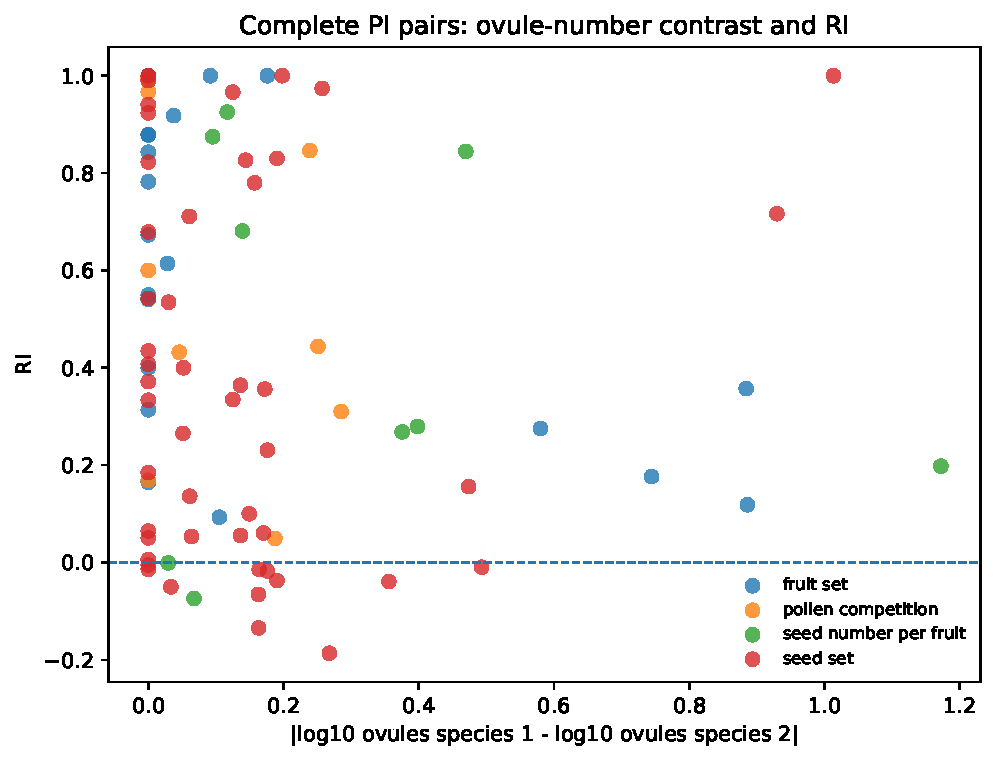
\includegraphics[width=0.80\linewidth]{../figures/fig8_ovule_difference_vs_RI.pdf}
\caption{Exploratory relationship between absolute log ovule-number contrast and RI in the complete PI subset.}
\end{figure}

\begin{table}
\caption{Descriptive correlations in the retained PI complete-case subset; these are diagnostics, not model tests.}
\label{tab:correlations}
\begin{adjustbox}{max width=\textwidth}
\begin{tabular}{lllll}
\toprule
x & y & n & pearson & spearman \\
\midrule
RI & K2P\_Distance & 87 & 0.206 & 0.322 \\
RI & mean\_log10\_ovules & 87 & -0.14 & -0.123 \\
RI & abs\_log10\_ovule\_difference & 87 & -0.116 & -0.214 \\
K2P\_Distance & abs\_log10\_ovule\_difference & 87 & -0.166 & -0.188 \\
\bottomrule
\end{tabular}
\end{adjustbox}
\end{table}


The directional test is biologically attractive because ovule number belongs to the maternal flower. For example, if the model predicts that a many-ovule maternal parent buffers cross failure, or alternatively exposes stronger post-pollination sorting, the reciprocal direction matters. The audit creates a file called \texttt{directional\_cleaned\_crosses.csv} with one row per maternal direction.

\begin{table}
\caption{Readiness of the reciprocal-direction data structure.}
\label{tab:directional_readiness}
\begin{adjustbox}{max width=\textwidth}
\begin{tabular}{llllll}
\toprule
subset & directions & complete\_without\_K2P & complete\_with\_K2P & complete\_PI\_with\_K2P & negative\_directional\_RI \\
\midrule
Retained Table1 directional rows & 1120 & 682 & 132 & 132 & 101 \\
\bottomrule
\end{tabular}
\end{adjustbox}
\end{table}


The directional structure is promising but uneven. In the retained data there are 1120 possible reciprocal directions, of which 682 have the interspecific outcome, maternal intraspecific baseline, and both ovule numbers. Only 132 also have K2P distance. Directional RI can be calculated as
\[
RI_{m,p} = 1 - \frac{C_{m,p}}{C_{m,m}},
\]
where \(C_{m,p}\) is the cross outcome with maternal species \(m\) and paternal species \(p\), and \(C_{m,m}\) is the intraspecific baseline for the maternal species. This definition is useful for diagnostics, but it inherits all problems of ratio data. It can be negative, it can exceed one if denominators are small or inconsistent, and it loses the original sampling variance.

\begin{figure}[H]
\centering
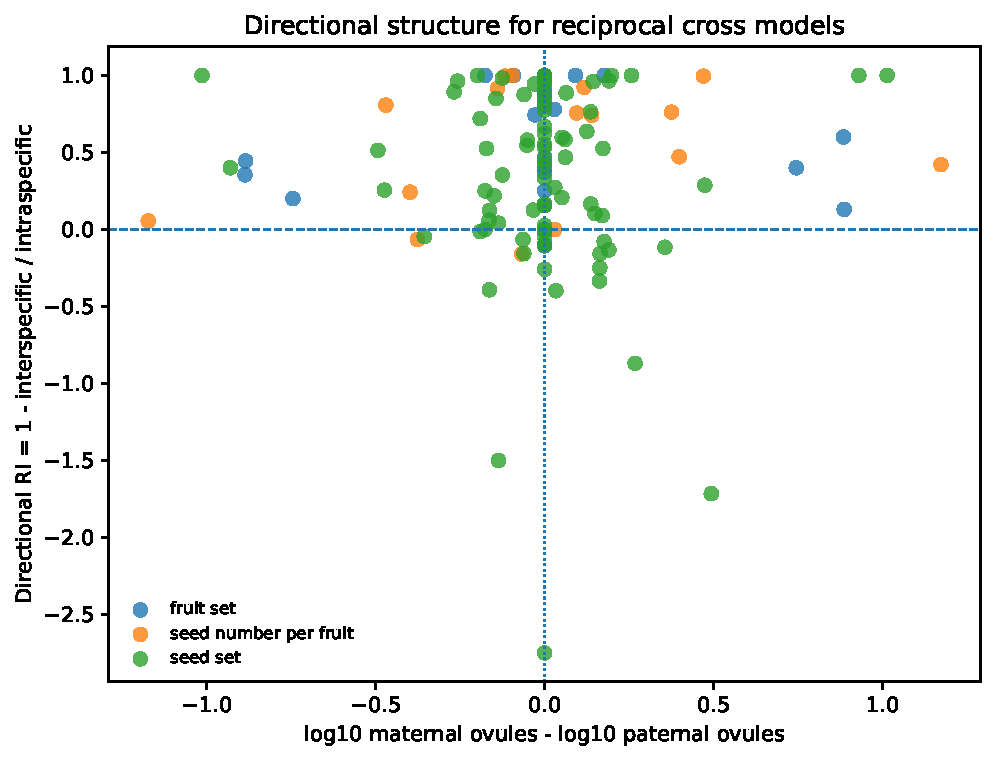
\includegraphics[width=0.80\linewidth]{../figures/fig10_directional_RI_by_ovule_ratio.pdf}
\caption{Directional RI against the signed maternal-paternal ovule-number contrast. The vertical line marks equal ovule numbers between maternal and paternal species.}
\end{figure}

\section*{Strengths of the datasets}

First, the project already separates response data from lineage-level covariates. That is good practice. Table 1 carries the pairwise RI and cross outcomes, while Table 2 carries ovule number, confidence, life history, and mating system. This separation makes joins explicit and allows uncertainty in ovule estimates to be modelled rather than hidden.

Second, the PI structure is coherent. The retained \texttt{PI\_name} values in Table 1 match the tree labels. This supports a conservative primary analysis based on the PI subset. It also makes it possible to compare three approaches: all retained rows, retained PI rows, and phylogenetic models using the full tree.

Third, reciprocal cross columns are present. This is important because ovule number is maternal in its immediate mechanism. A pair-level RI index can test whether species-pair contrasts matter, but reciprocal cross data can test whether the maternal side of the contrast matters.

Fourth, confidence categories are available for ovule number. This is useful for sensitivity analysis. A model fitted to all numeric ovule estimates can be compared with a stricter model using only confidence categories 1--2 or 1--3.

Fifth, the prospective templates are pointed in the right direction. The lineage template includes ovules, pollen production, pollen load, stigma size, style length, mating system, pollination syndrome, and flowering time. The cross template includes flower counts, ovules exposed, seeds matured, fruit set, pollen dose, pollen-tube information, F1 viability, F1 fertility, and genetic distance. Those fields would allow a much stronger count-level model than the current aggregated RI table.

\section*{Weaknesses and consequences for the model}

The main weakness is that the effective sample size drops when the biologically strongest conditions are imposed. A PI complete-case model with both ovule numbers and K2P distance has 87 rows. This is sufficient for a simple analysis, but not for a saturated model with multiple interactions and random effects. A good first analysis should therefore test a small number of contrasts: genetic distance, absolute ovule-number difference, mean ovule number, and measurement type.

The second weakness is measurement heterogeneity. RI values derived from fruit set, seed set, seed number per fruit, and pollen competition do not share the same denominator. This affects the meaning of the slope. If ovule number predicts seed number per fruit but not fruit set, then pooling the responses may obscure the mechanism. Treat measurement type as a fixed effect, fit stratified models as sensitivity checks, or use a hierarchical model with measure-specific intercepts and slopes.

The third weakness is the loss of denominator information. Aggregated RI values hide the number of flowers, ovules, fruits, or seeds behind each estimate. This matters because an RI value based on 20 crosses should not carry the same precision as an RI value based on 500 crosses. The future cross-level template solves this. For the current data, use robust standard errors, nonparametric bootstrap over pairs, and sensitivity analyses by measurement type and confidence.

The fourth weakness is missing and uncertain ovule data. Table 2 has 97 missing ovule numbers, and some large estimates have low confidence. The practical consequence is that complete-case analyses may be biased if missingness is phylogenetically or biologically structured. Use confidence-weighted sensitivity analyses and consider multiple imputation, but do not let imputation create false precision. Report complete-case and imputed results side by side.

The fifth weakness is the response scale. The RI column ranges from -0.8968 to 1.0000, with 59 negative values. Negative values are biologically meaningful because they indicate interspecific performance exceeding the intraspecific baseline. Boundary values at 1 are also present. A standard beta regression is therefore not valid on raw RI without transformation or censoring. Prefer models on log relative success where possible, or use Gaussian/robust models for RI with careful residual checks.

The sixth weakness is tree-label duplication. A duplicated \texttt{Corymbia} tip may break phylogenetic covariance construction. This is easy to fix, but it must be fixed before using tools such as \texttt{ape}, \texttt{phylolm}, \texttt{MCMCglmm}, \texttt{brms}, or \texttt{RevBayes}.

\section*{Suggested analysis tools}

For the current pair-level data, start with a transparent R or Python pipeline that creates a single analysis table. The minimum columns are species pair, \texttt{PI\_name}, RI, measure, both ovule numbers, ovule confidence categories, life history, mating system, and K2P distance. The file \texttt{model\_ready\_PI\_pairs.csv} created by this audit is a first version of that table.

For simple first-pass models, use linear models or robust linear models on RI, with \(\Delta O\), mean log ovule number, K2P distance, and measurement type as predictors. This gives a readable baseline. Follow this with permutation or bootstrap intervals over PI pairs. The bootstrap should resample pairs, not rows nested within the same pair.

For phylogenetic sensitivity, use phylogenetic generalised least squares. In R, \texttt{ape} can read and clean the Newick tree, \texttt{caper} or \texttt{nlme} can fit PGLS-style models, and \texttt{phylolm} can fit phylogenetic linear models. If you need measurement-error models or crossed random effects, use \texttt{brms} with a phylogenetic covariance matrix. The PI subset should remain the primary check because it is easy to explain.

For reciprocal cross models, reshape the data into maternal-direction rows. A useful diagnostic response is \(\log(C_{m,p} + c) - \log(C_{m,m} + c)\), where \(c\) is a small offset chosen before looking at the results. The key predictor is \(D_{m,p} = \log_{10}(O_m)-\log_{10}(O_p)\). Include pair as a clustering unit. If raw counts become available, replace the ratio response with a binomial, beta-binomial, Poisson, negative-binomial, or hurdle model depending on the denominator and outcome.

For missing ovule numbers, first report complete-case results. Then run sensitivity analyses using confidence thresholds: all numeric estimates, confidence 1--3, and confidence 1--2. Multiple imputation can be useful, but it should include genus, family, life history, mating system, and phylogenetic information. Imputation should not be used as the only analysis.

For future data collection, use the supplied templates but keep count denominators. The most useful fields are flowers crossed, ovules exposed, seeds matured, fruits formed, pollen dose, pollen tubes reaching the ovary, F1 viability, and F1 fertility. These allow the model to distinguish three stages: pollination success, seed maturation, and later hybrid fitness. That distinction is where the ovule-number model can become mechanistic rather than purely comparative.

\section*{Recommended next steps}

The immediate next step is to verify the PI flag. Add an explicit \texttt{is\_PI} column to Table 1 and keep \texttt{PI\_name} as the tree label. Then collapse duplicate genetic-distance rows and decide how to treat the 23 missing K2P values. Next, inspect the largest ovule-number estimates, especially low-confidence values, because they can dominate log-scale diagnostics less than raw-scale fits but still affect leverage.

After that, fit three models in order. First, fit a complete-case PI pair-level model with RI as the response. Second, repeat the model under stricter ovule-confidence thresholds. Third, fit a directional reciprocal-cross model using \texttt{directional\_cleaned\_crosses.csv}. The directional model is the most biologically informative, but the pair-level model is the safest first test.

\conclusionbox{\textbf{Bottom line.} The datasets are strong enough for a careful first paper-level analysis, provided the claims are framed around a conservative PI complete-case test and sensitivity analyses. The strongest future version of the project would move from aggregated RI to count-level reciprocal crosses, because ovule number is a denominator and a maternal trait, not just a lineage-level covariate.}

\appendix
\section*{Additional structural tables}

\begin{table}
\caption{Summary of the ovule-number master table.}
\label{tab:master_summary}
\begin{adjustbox}{max width=\textwidth}
\begin{tabular}{ll}
\toprule
quantity & count \\
\midrule
Rows in master table & 5496 \\
Rows marked table1 == yes & 1208 \\
Rows marked for removal & 832 \\
Nonremoved rows & 4664 \\
Nonremoved rows with ovule number & 4206 \\
Unique nonremoved species names & 3779 \\
Unique nonremoved table1 species names with number & 711 \\
\bottomrule
\end{tabular}
\end{adjustbox}
\end{table}


\begin{table}
\caption{The 20 columns with nonzero missingness shown first by dataset.}
\label{tab:missingness_top20}
\begin{adjustbox}{max width=\textwidth}
\begin{tabular}{llll}
\toprule
dataset & column & missing & missing\_percent \\
\midrule
Genetic distances & K2P\_Distance & 23 & 16.3 \\
Table1 & sp2\_hybrid\_proportion & 559 & 96.7 \\
Table1 & sp1\_hybrid\_proportion & 556 & 96.2 \\
Table1 & PI\_name & 437 & 75.6 \\
Table1 & interspecific\_value\_sp2\_sp1 & 145 & 25.1 \\
Table1 & intraspecific\_value\_sp2 & 121 & 20.9 \\
Table1 & interspecific\_value\_sp1\_sp2 & 87 & 15.1 \\
Table1 & intraspecific\_value\_sp1 & 73 & 12.6 \\
Table2 & ovule\_number & 97 & 23.8 \\
Table2b & Remove & 4664 & 84.9 \\
Table2b & number & 468 & 8.5 \\
Table2b & family & 11 & 0.2 \\
Table2b & genus & 11 & 0.2 \\
Table2b & level & 11 & 0.2 \\
\bottomrule
\end{tabular}
\end{adjustbox}
\end{table}


\begin{figure}[H]
\centering
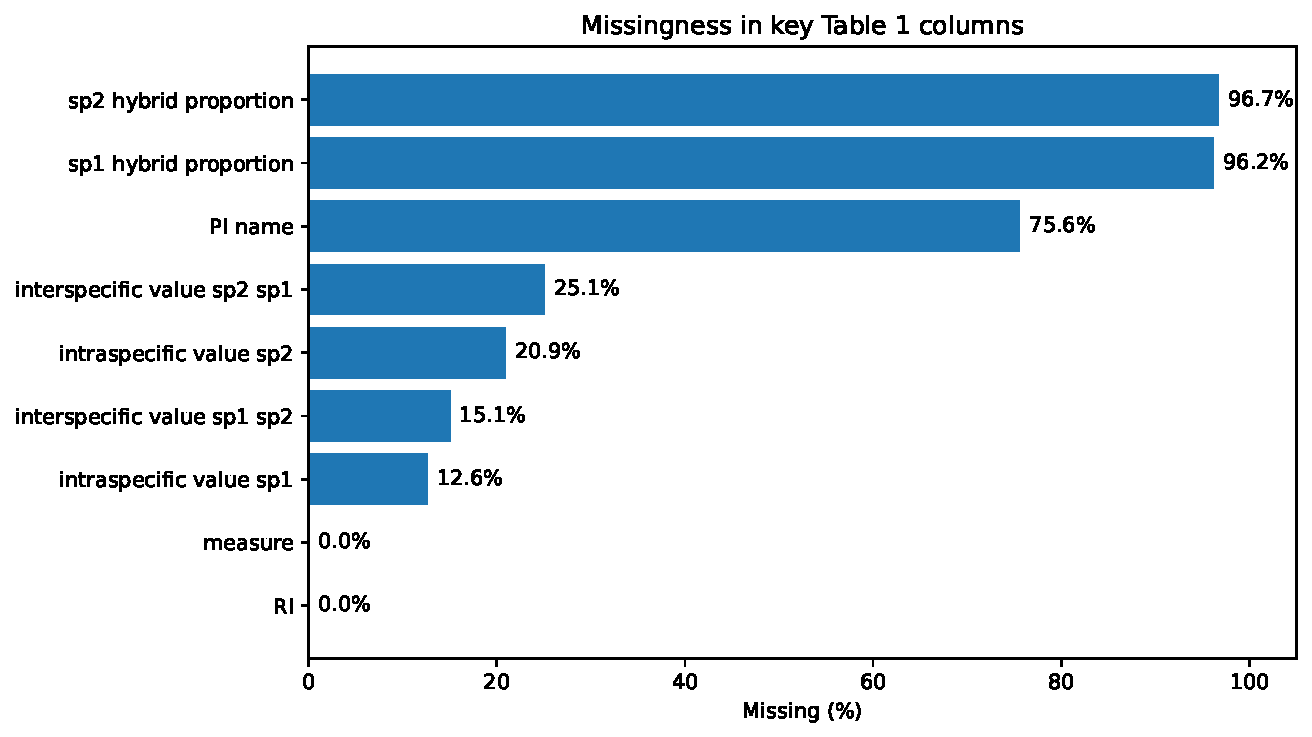
\includegraphics[width=0.90\linewidth]{../figures/fig3_table1_missingness.pdf}
\caption{Missingness in key Table 1 fields. Hybrid-proportion columns are sparse because they apply mainly to pollen-competition rows.}
\end{figure}

\begin{figure}[H]
\centering
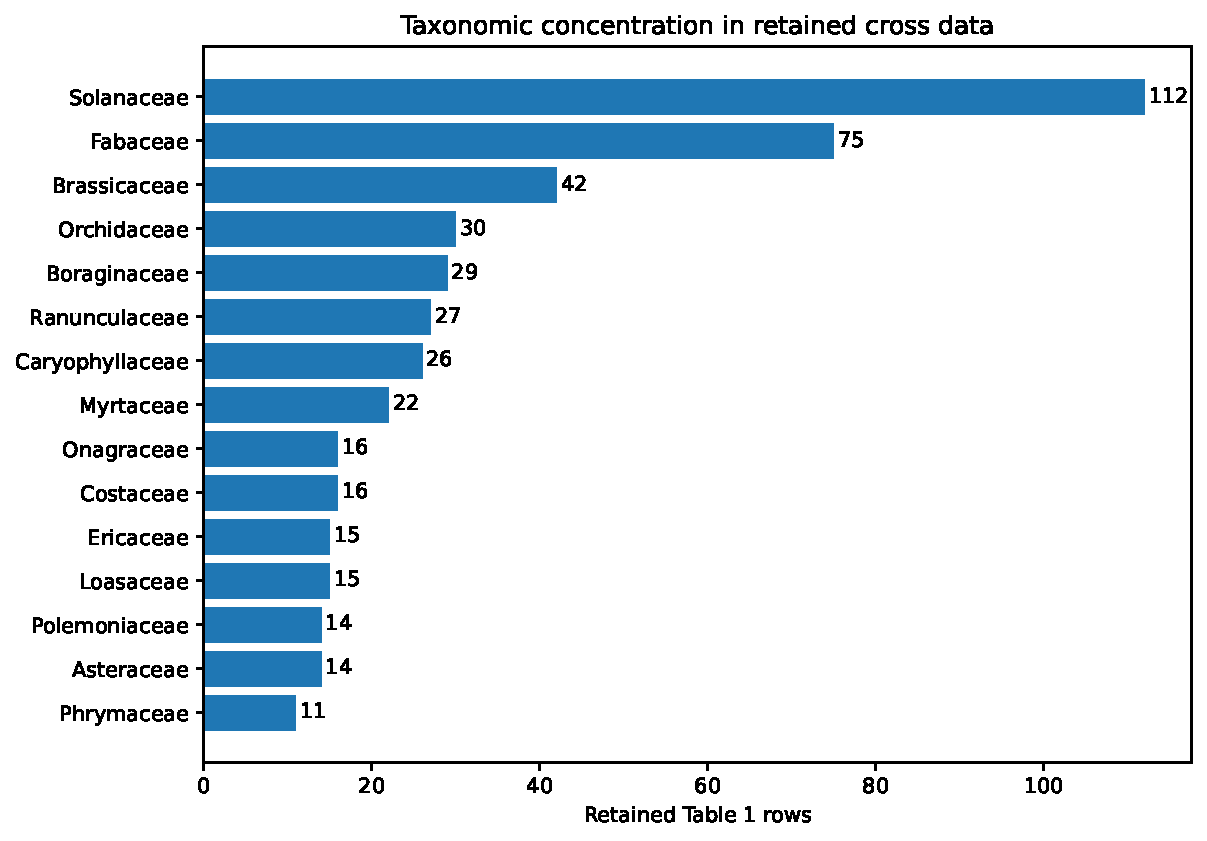
\includegraphics[width=0.86\linewidth]{../figures/fig9_family_coverage.pdf}
\caption{Retained Table 1 rows are concentrated in a subset of plant families. This should be considered when interpreting broad comparative claims.}
\end{figure}

\end{document}
